\begin{bibunit}
	
\rhead{\thepage}

\chapter{Introduction}
Urban development drastically changes the character of the surface. Replacement of natural terrain with roads, buildings, parks, and other urban features modifies the geometry of the surface as well as its thermal, radiative, moisture, and aerodynamic properties. These modifications, combined with anthropogenic emissions of heat, result in a distinct urban climate; one which is often warmer, a phenomenon termed the urban heat island effect (UHI). As both the Earth's population and the urbanized fraction of that population increase \citep{Nations2014}, cities grow and more people are exposed to urban-modified atmospheres. Thus, understanding how cities interact with the climate across spatiotemporal scales has important implications for human health, energy efficiency, and for informing future urban development. This, in part, has prompted significant expansion in study of the urban effect on climates, with particular focus on characterization of the urban effect on surface (T\textsubscript{surf}) and air (T\textsubscript{air}) temperatures.

\pagebreak

The temperature of a surface (urban or otherwise) at its interface with the atmosphere is defined as the net result of the surface energy balance \citep{Oke2017}, wherein change in temperature at time $t$ for a surface with thickness $z$ and heat capacity $C$ can be solved as,

\begin{equation}
	C~\frac{\partial \text{T\textsubscript{surf}}}{\partial t}~z = Q^*+ Q_F - Q_H - Q_E - \Delta Q_A - \Delta Q_G
\end{equation}

\noindent where $Q^*$ is net radiation at the surface, $Q_F$, $Q_H$, and $Q_E$ are fluxes of anthropogenic, sensible, and latent heat, $\Delta Q_A$ is net advection of surface heat to or from the volume of air above the surface, and $\Delta Q_G$ is net storage of heat by the substrate below. A change in T\textsubscript{surf} is translated to change in T\textsubscript{air} as the surface exchanges energy with the atmosphere above it, primarily via convection and radiation. As such, T\textsubscript{surf} and T\textsubscript{air} are inextricably linked, particularly near to the ground, and a city's altered surface characteristics and energy balance manifest in modifications to both surface and air temperature regimes.

%While most study of urban effects on climate is concentrated on analysis of urban air temperatures, the linkage between the two, and an increased focus on the importance of the surface in boundary-layer climatology, has also  Knowledge of how cities interface with and modify climates can come through study of the urban effect on both surface and air temperatures.

%As accurate characterization of all of the terms of the energy balance is difficult and plagued by uncertainties and closure problems, characterization of how cities affect the \textit{net result} of energy balances at and near the surface - via characterization of the urban effect on air and surface temperatures - provides a viable alternative for understanding how cities interface with and modify climate.

%The relationship between the temperature of the surface and the temperature of the air is complex, particularly in cities, and poorly understood. 

The notion that urban modifications to the environment produce elevated T\textsubscript{air} and T\textsubscript{surf} is not new, with the first formal studies of the urban effect on T\textsubscript{air} dating back to \citet{Howard1833}'s identification of "artificial warming" and "urban contamination" in his characterization of spatial patterns of T\textsubscript{air} in early 19\textsuperscript{th} century London. Conceptually, contemporary studies of urban climate do not stray far from \citet{Howard1833}, by seeking to isolate and quantify the urban signal in measured or modeled assessment of a given meteorological variable. However, as \citet{Howard1833} identified nearly two centuries ago, the sheer number of factors influencing direct measurement of climates makes experimental control nearly impossible in observational study. In any given observation of climate, myriad urban and non urban signals make it difficult to reliably differentiate urban influenced measures from those free of urban influence, degrading interstudy comparison. Development of physically based numerical models to represent physical processes affected by urbanization, and which permit experimental control, have shown promise \citep{Krayenhoff2014,Gastellu-Etchegorry1996,Masson2000,Martilli2002} yet the inherent complexity in simulating flows of energy, momentum and mass at the scales necessary to represent the full range of physical processes over realistic environments remains an on-going challenge. Thus, accurate assessment of how a city affects the climate is a deceptively challenging task. To address this, \citet{Lowry1977} presents a framework to isolate the urban effect in observation of a given meteorological variable. In his framework - termed the "Lowry method" - measurement of a meteorological variable ($V_M$) is the sum of forcings from the background climate and synoptic conditions ($V_B$), local topography ($V_L$), and the urban landscape ($V_H$)

\begin{equation}
	V_M = V_B + V_L + V_H
\end{equation}

Thus, isolation of the urban effect on observed $V_M$ simply requires the removal of $V_B$ and $V_L$. This can be achieved by subtracting some urban affected observation ($V_{M, \ U}$) from a non-urban observation ($V_{M, \ R}$) where $V_{H, \ R}$ = 0,

\begin{equation}
V_{M, U} - V_{M, R} = (V_B + V_L + V_H) - (V_B + V_L) = V_H
\end{equation}

\noindent simplified as,

\begin{equation}
	V_H = V_{M, \ U} - V_{M, \ R}
\end{equation}

Study of the UHI with respect to T\textsubscript{air} (aUHI) - typically referring to T\textsubscript{air} measured from approximately 2 \si{\meter} above ground level, yielding a "canopy layer" UHI (sUHI) - and T\textsubscript{surf} (sUHI) tacitly falls into such a framework, by replacing $V_{M, \ U} - V_{M, \ R}$ with $\Delta$T\textsubscript{U - R}. However, in spite of its conceptual simplicity through the lens of the Lowry method, meta-analysis of observational aUHI studies suggests that that simplicity may not translate well to real world analysis. In a points based assessment of 190 aUHI studies published between 1950 and 2007, \citet{Stewart2011} found that nearly 50\% of studies are "scientifically indefensible". In his analysis, each study was given a "passing" or "failing" grade and ranked based on methodological quality in the following criteria: conceptual model, operational definitions, instrument specification, site metadata, site representativeness, number of replicates, weather control, surface control, and synchronisity. Of the 190 surveyed studies, only 13\% were derived from field sites that were sufficiently representative of the local-scale environment or lacked the meta-data to make such a determination, leading to potential biases from micro-scale terrain. 89\% lacked meta-data altogether. These findings suggest a significant gap between conceptual simplicity and practical realities in UHI analysis.

Conceptual problems in the aUHI literature are particularly discouraging as they are not the result of an evolution in measurement techniques or improved instrumentation. Techniques to observe and analyze aUHI did not see significant evolution in the period between 1950 and 2007 - in fact, \citet{Stewart2011} suggests the opposite: a disproportionately large number of studies deemed scientifically sound were published early in the study purview. In the five years since its publication, aUHI study has seen further expansion and, as such, it is difficult to assess whether its critical analysis has prompted a shift towards more thoughtful, careful, and methodical study of aUHI, notwithstanding its relevance in study of the urban effect on other meteorological variables. Thus, in study of the urban effect on variables for which significant methodological shifts have or will occur, the warnings implicit in \citet{Stewart2011} are particularly salient, as inherent difficulties found in translating "Lowry"-esque conceptual models to real world observations may be compounded by significant methodological changes. What is clear in light of these findings, however, is that assessment of the urban effect on climate is \textit{fundamentally difficult} in spite of its conceptual simplicity. 

%In the context of assessment of the urban effect on T\textsubscript{surf} assessment, where new techniques, instruments, and add significant complexity, critical assessment of both conceptual and methodological shortcomings should accompany assessment of biases in different measurement and modeling techniques. 

In contrast to urban T\textsubscript{air} and aUHI assessment, where measurement techniques have not undergone significant recent evolution and methodological problems arise in large part from conceptual shortcomings and simple carelessness, study of the urban effect on land T\textsubscript{surf} is relatively new and significantly more complex. As such, methodological problems in sUHI study can arise from both conceptual flaws \textit{and} instrument biases. In spite of these difficulties, the introduction of new methods, instruments, and analytical techniques in TIR remote sensing of urban environments has lead to rapid proliferation in study of urban T\textsubscript{surf} and the sUHI - much of which is focused on remote sensing of upwelling thermal infrared radiation (TIR). In the decades preceding this thesis, a combination of factors has lead to an increased focus on remote sensed study of urban T\textsubscript{surf}: 

\begin{itemize}
	\item The proliferation of satellite and aerial TIR remote sensors and "openness" in data access policies.
	\item Improvements in sensor spatial, spectral, and radiometric resolutions. 
	\item An increased focus on the importance of the surface in both determining and understanding key near-ground micro-meteorological phenomena.
	\item Interest in T\textsubscript{surf} for human thermal comfort, energy conservation, and sUHI mitigation applications. 
\end{itemize}

Remote sensed study of the urban effect on land T\textsubscript{surf} has been critical in characterizing large-scale spatial and temporal patterns of sUHI \citep{Peng2012, Streutker2003, Imhoff2010}. However, the methodological and conceptual concerns raised in \citet{Stewart2011} in combination with the wide (and broadening) range of methodologies for remote sensed urban T\textsubscript{surf} retrieval should prompt critical assessment of the remote sensed sUHI literature. At the time of writing, no systemic or critical reviews of the remote sensed sUHI literature are available. In addition, an increasingly dogmatic focus on improving spatial and radiometric resolutions has left other biases inherent in remote sensing of urban environments largely ignored in sUHI literature. This suggests that similar conclusions to those found of aUHI literature in \citet{Stewart2011} are possible (if not likely) for study of sUHI. Assessment of these biases is, therefore, paramount to ensure assessments of the urban effect on T\textsubscript{surf} are robust, methodologically valid, and comparable across techniques, space, and time.

\section{Biases and shortcomings in thermal remote sensing of urban T\textsubscript{surf}}

Traditional methods for urban T\textsubscript{surf} measurement are subject to a suite of geometric and temporal biases. Geometric biases are the result of urban modification of surface structure and thermal and radiative properties combined with the  narrow field-of-view (FOV) viewing geometry of conventional remote sensors:

%These biases are largely inherent to the discipline and contribute an additional source of error on top of potential concerns carried over from meta-analysis of conceptual flaws in aUHI literature. 

\subsection*{\textnormal{\textit{Undersampling of surface 3-dimensionality by narrow-FOV remote sensors}}}

Relative to typical non-urban and rural terrain, urban development adds significant 3-dimensionality to the surface. This added complexity results in undersampling of the complete urban surface by narrow-FOV remote sensors. A narrow-FOV sensor "sees" a different assemblage of urban surfaces depending on its viewing direction, resulting in a geometric bias towards some arrangement of facets; i.e. viewing from the nadir, a narrow-FOV sensor sees the urban surface as an array of rooftops and roads, the same sensor viewing the surface from an oblique angle sees some array of walls, rooftops, and roads depending on its orientation. For a sensor in the nadir, increasing FOV introduces sampling of vertical features. To illustrate how sensor-surface geometry influences sampling of the urban surface by narrow- and wide-FOV sensors, Figure \ref{model} shows FOVs for the three sensor orientation/type combinations.The vast majority of urban thermal remote sensing is done via a narrow-FOV sensor viewing from the nadir.

\begin{figure}[H]
	\centering
	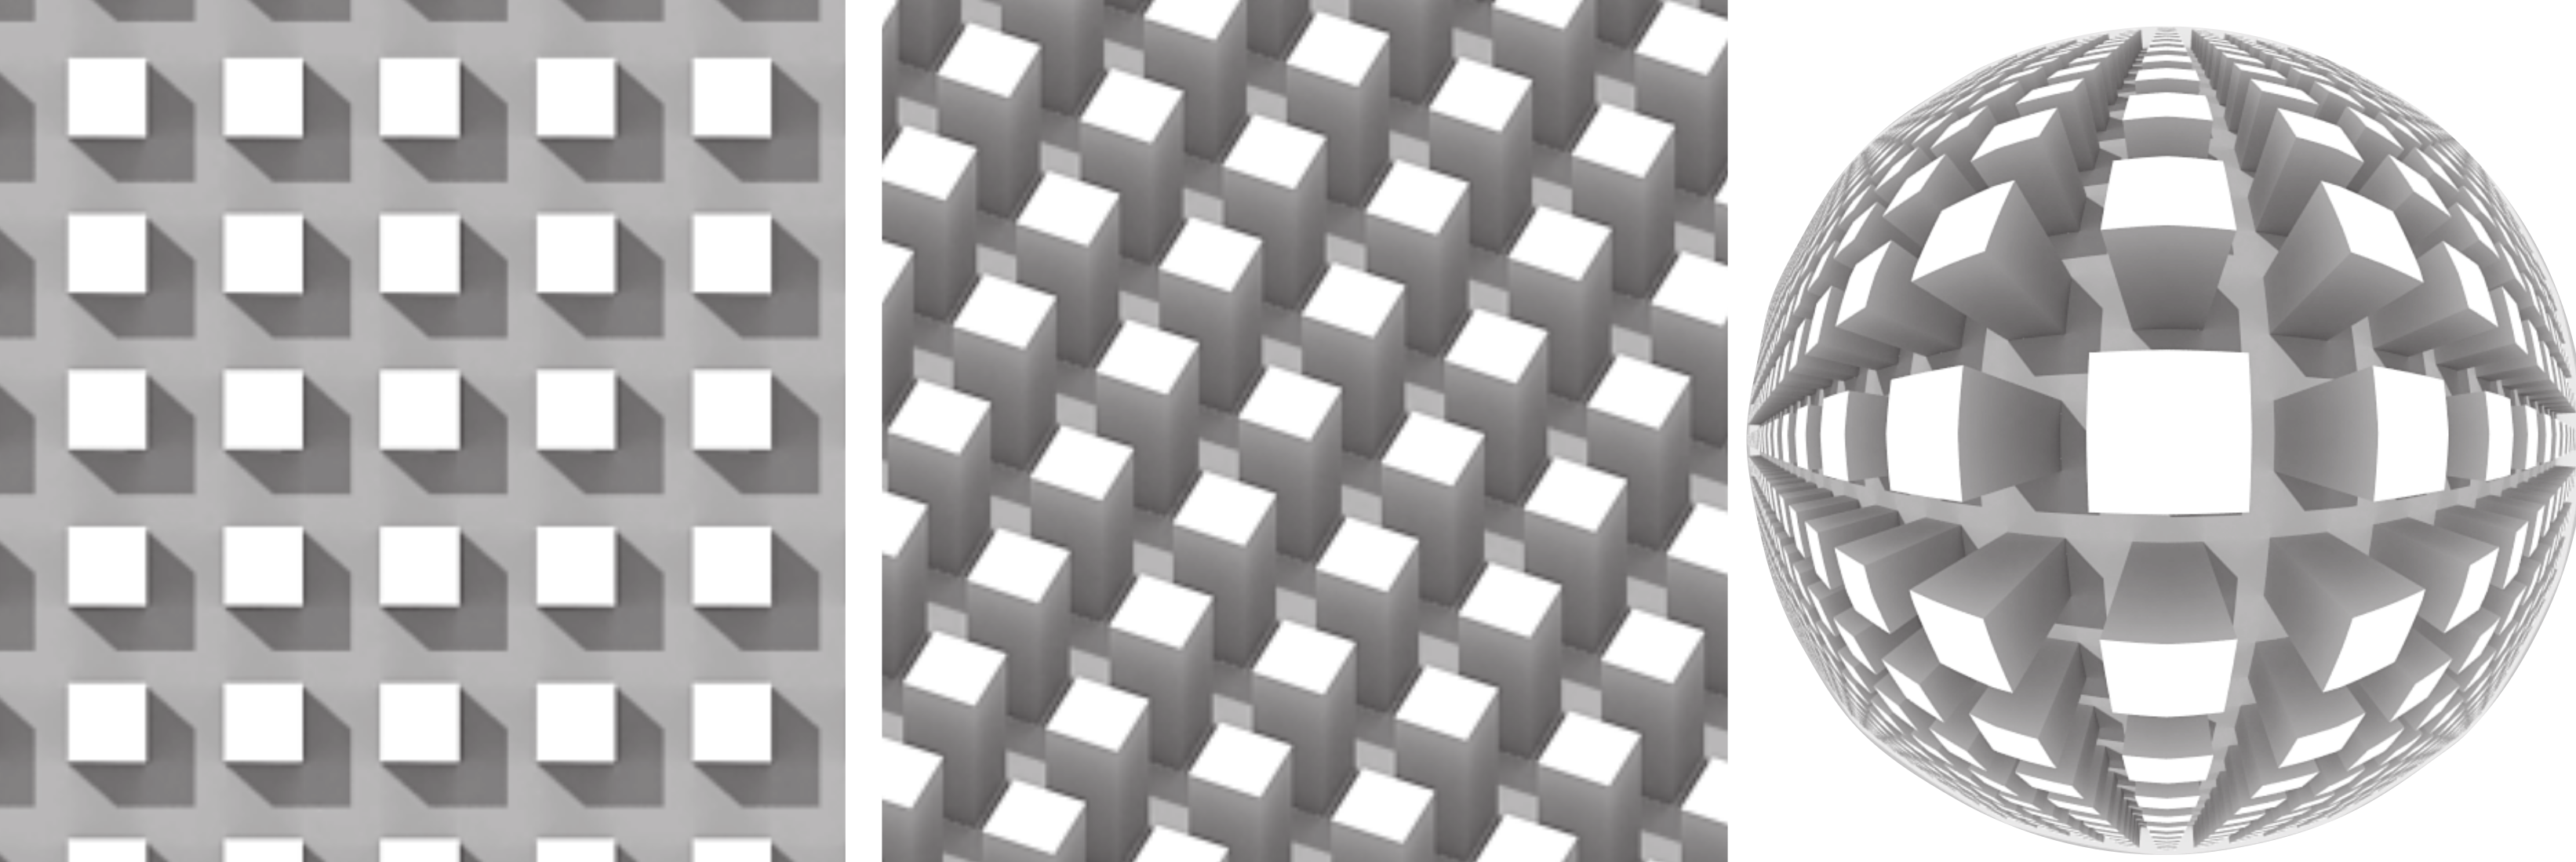
\includegraphics[width=15cm,
	height=7in,
	keepaspectratio]{model}
	\caption{Projected FOVs for a narrow-FOV sensor at nadir and oblique angles, and a wide-FOV hemispherical sensor viewing an idealized urban array with building width \textit{H}, height 2\textit{H}, and inter element spacing \textit{H}. Figure from \cite{Adderley2015}.}
	\label{model}
\end{figure}

\subsection*{\textnormal{\textit{Directional dependence in remote sensed urban T\textsubscript{surf}}}}

In addition to modifying how a remote sensor samples the surface, the convoluted 3-dimensional structure of the urban surface modifies the surface radiation budget, resulting in strong micro-scale spatiotemporal contrasts in urban T\textsubscript{surf}, which depend on surface-sun geometry. These microscale variations in urban T\textsubscript{surf} are often amplified by significant geometric and spatial contrasts in the thermal admittance of common urban materials, which determines the diurnal amplitude of T\textsubscript{surf} for a given facet. Thus, when viewed from a narrow-FOV remote sensor with some inherent geometric bias, urban T\textsubscript{surf} is directionally dependent - constituting an "effective anisotropy" of urban T\textsubscript{surf}, shown in Figure \ref{anisot}. The qualifier "effective" is used to differentiate directional contrasts in urban T\textsubscript{surf} that arise from a city's 3-dimensional surface structure from those resulting from the non-Lambertian nature of individual urban facets (e.g. walls, rooftops, or roads). The magnitude of urban effective anisotropy can reach up to 10 \si{\kelvin} and is highly dependent on surface-sensor-sun geometry, surface structure, and urban materials \citep{Krayenhoff2016, Voogt1997}. 

\begin{figure}[H]
	\centering
	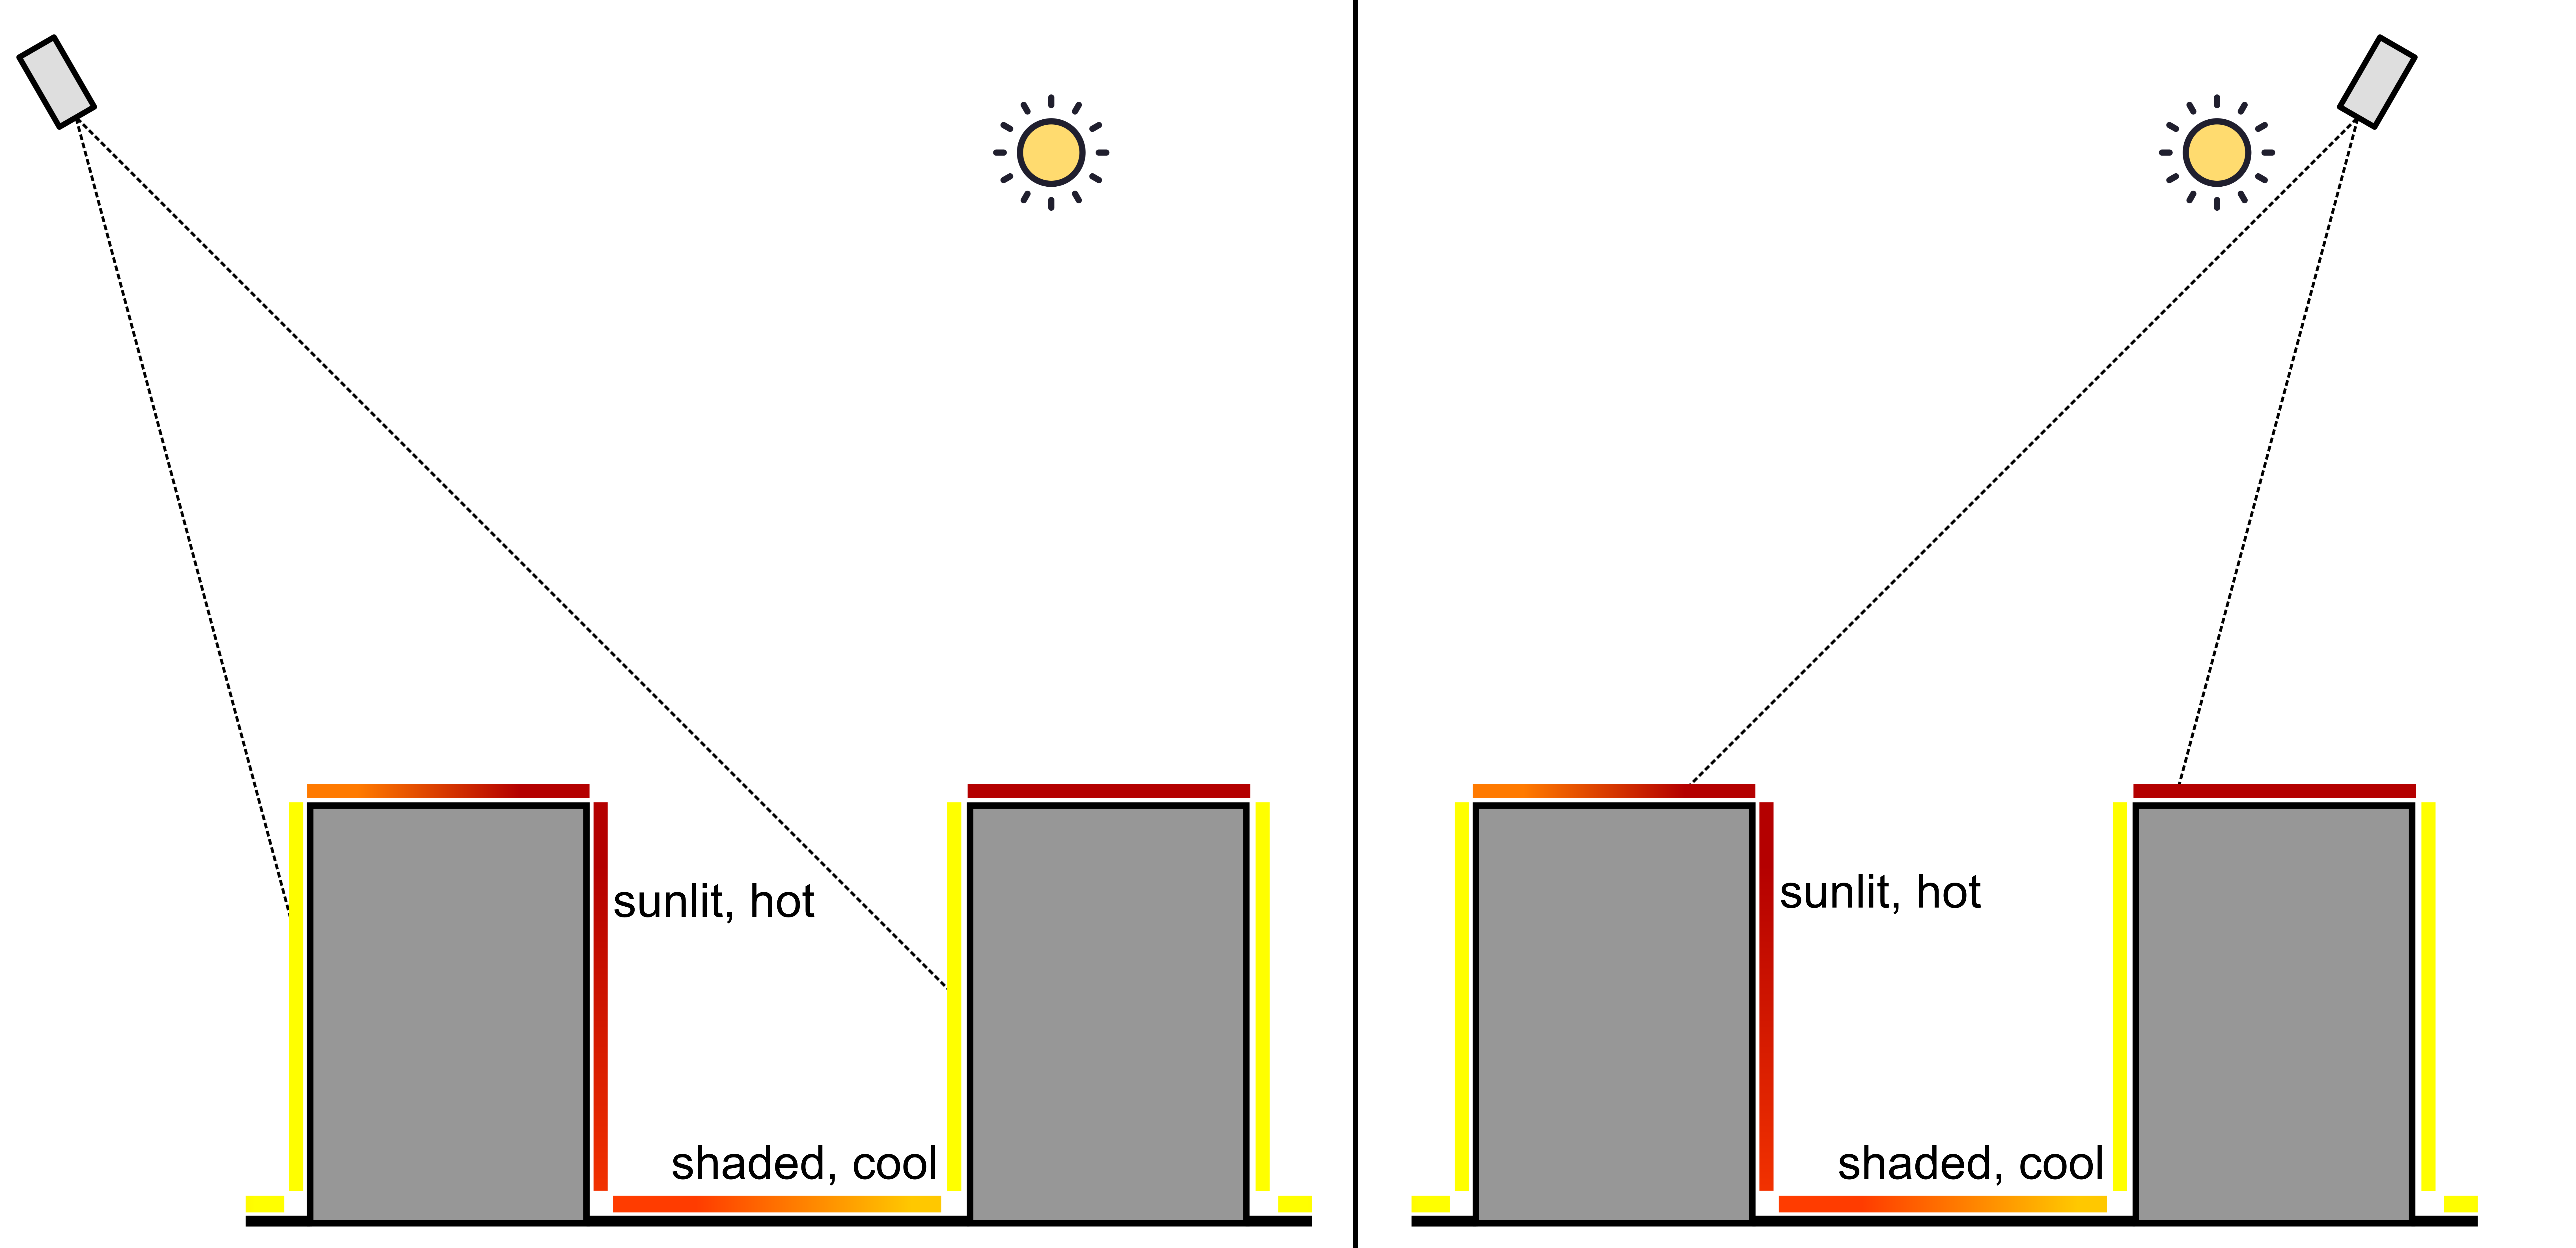
\includegraphics[width=15cm,
	height=7in,
	keepaspectratio]{anisot}
	\caption{A narrow-FOV sensor viewing an idealized urban surface from two angles. Left: viewing the surface approximately perpendicular to the sun's angle. Right: viewing the surface approximately parallel to the sun's angle. The two viewing angles yield different remote sensed T\textsubscript{surf} by sampling different arrangements of sunlit and shaded features. Both will deviate from an area weighted "complete" urban T\textsubscript{surf}.}
	\label{anisot}
\end{figure}

Geometric undersampling by narrow-FOV remote sensors results in remote sensed urban T\textsubscript{surf} changing based on a sensor's viewing direction and the assemblage of facets included within the sensor FOV. A sensor viewing the surface perpendicular (parallel) to the sun's angle will tend to underestimate (overestimate) the "true" complete urban surface temperature - often calculated as an area weighted average of wall, rooftop, and road T\textsubscript{surf} - by differentially biasing sunlit or shaded facets. Similarly, a sensor in the nadir will tend to overestimate daytime urban T\textsubscript{surf} and underestimate nighttime T\textsubscript{surf}, from a bias towards differentially hot (cool) rooftop facets by day (night) and a neglect of wall facets which are differentially cooler (warmer) by day (night). As the effect of geometric biases is highly dependent on surface-sensor-sun geometry and requires significant instrumentation for quantification, its influence in the remote sensed sUHI record is presently unknown.

Temporal biases in thermal remote sensing of urban areas occur across multiple time scales including: 
\subsection*{\textnormal{\textit{Contamination by turbulence forced, high frequency fluctuations in urban T\textsubscript{surf}}}}

Using time-sequential thermography \citet{Christen2012} found that many common urban fabric types (e.g. rooftops, walls, roads, and vegetation) display large micro-scale (second to minute) fluctuations in T\textsubscript{surf}. The magnitude of these is inversely related to surface thermal admittance and is currently, poorly understood. Most thermal remote sensors provide instantaneous, rather than temporally averaged, T\textsubscript{surf} and thus are subject to contamination by high-frequency fluctuations. These biases are difficult to estimate in urban environments, where a large variety of fabric materials can produce significant geometric and spatial contrasts in thermal admittance --- and thus directional and spatial variations in the magnitude of microscale fluctuations depending on the facet material types viewed by the sensor. 

\subsection*{\textnormal{\textit{Discontinuity in satellite overpass cycles.}}}

Overpass cycles for polar orbiting sensors are discontinuous. These sensors provide data for the vast majority of urban T\textsubscript{surf} study. Assessment of land T\textsubscript{surf} either sacrifices spatial resolution for a daily repeat cycle - as is the case with MODIS  - or sacrifices temporal resolution for a higher spatial resolution - ASTER or Landsat. These satellites cannot be used to assess the temporal development of sUHI without significant interpolation. Geostationary satellite sensors overcome this limitation but low spatial resolutions limit applicability in urban areas, especially at mid to high latitudes. 

\subsection*{\textnormal{\textit{Clear-sky bias}}}

Clouds absorb TIR - thus satellite TIR remote sensing of the surface requires clear sky conditions. Although the urban effect on T\textsubscript{surf} is most evident under "satellite friendly" clear sky conditions (manifesting as large sUHI magnitudes), a clear sky bias likely entails overestimation of "all-sky" sUHI and further adds to discontinuities in the remote sensed urban T\textsubscript{surf} record.

As is the case with geometric biases, the magnitude of these temporal biases in remote sensed urban T\textsubscript{surf} is difficult to quantify without long-term ground truthing campaigns or significant interpolation. As such, the true temporal and geometric nature of urban effect on T\textsubscript{surf} and thus sUHI is presently unknown.
 
\section{Research questions and objectives}

Prompted by these shortcomings in the remote sensed urban T\textsubscript{surf} record, and in an effort to better understand the temporal and geometric aspects of sUHI, this thesis introduces a method to provide hemispherical, temporally continuous urban T\textsubscript{surf} for sUHI analysis to address the following questions:

\begin{enumerate}
	\item What is the nature of urban surface temperature when viewed from a hemispherical downward-facing radiometer? And how does it relate to urban temperatures derived from other methods for urban surface temperature retrieval?
	\item What is the diurnal and seasonal nature of the surface urban heat island effect?
\end{enumerate}

\noindent In an attempt to answer these questions, this thesis

\begin{itemize}
	\item Develops and evaluates a method to retrieve atmospherically correction hemispherical radiometric urban surface temperatures from time-continuous measurements of upwelling longwave radiation.
	\item Compares urban surface temperatures and surface urban heat island magnitudes retrieved using the method to common remote sensed representations of the urban surface.
	\item Derives two long term climatology of hemispherical urban surface temperatures to observe seasonal and diurnal patterns of the surface urban heat island effect.
\end{itemize}

The following two chapters address questions one and two respectively. Chapter \ref{paper1} details and evaluates a method to retrieve atmospherically corrected, hemispherical urban T\textsubscript{surf} from time-continuous measurements of upwelling longwave radiation. Chapter \ref{paper2} explores the temporal and geometric nature of sUHI through long-term climatological analysis of hemispherical sUHI and compares sUHI magnitudes from several representations of the urban surface.


\cleardoublepage 
\phantomsection  
\renewcommand*{\bibname}{References}
\addcontentsline{toc}{section}{\textbf{References}}

\putbib
\end{bibunit}